
All five sub-hypotheses passed their gates. Results are reported in RQ order.

\subsubsection{5.1 RQ1: Capability Independently Predicts LC Preference (H-E1)}

After controlling for avg\_length:

> \textbf{r\_partial = 0.9851, p = 1.69e-170 (one-tailed), bootstrap 95\% CI [0.976, 0.988], N = 223}

VIF = 1.764 confirms no multicollinearity. Figure 1 shows the bivariate scatter (Spearman $\rho$ = 0.966); Figure 2 shows the partial regression plot after residualizing avg\_length.

The partial correlation (0.985) exceeds both the bivariate correlation in the present sample (0.966) and the previously reported bivariate of 0.94 \citep{Dubois2024LengthControlled}. Verbosity acts as a mild suppressor: capable models write somewhat longer responses, which partially masks the true capability-LC signal in bivariate analysis. After residualization, the capability signal dominates. Figure 3 (bootstrap distribution) confirms stability across 1000 resamples.

\begin{table}[htbp]
\centering
\resizebox{\columnwidth}{!}{%
\begin{tabular}{llll}
\toprule
Metric & Value & Threshold & Status \\
\midrule
r\_partial & 0.9851 & $\geq$ 0.15 & EXCEEDED \\
p-value & 1.69e-170 (one-tailed) & < 0.05 & EXCEEDED \\
Bootstrap CI lower & 0.976 & > 0 & CONFIRMED \\
VIF & 1.764 & < 5.0 & MET \\
\bottomrule
\end{tabular}
}
\end{table}

\begin{figure}[htbp]
\centering
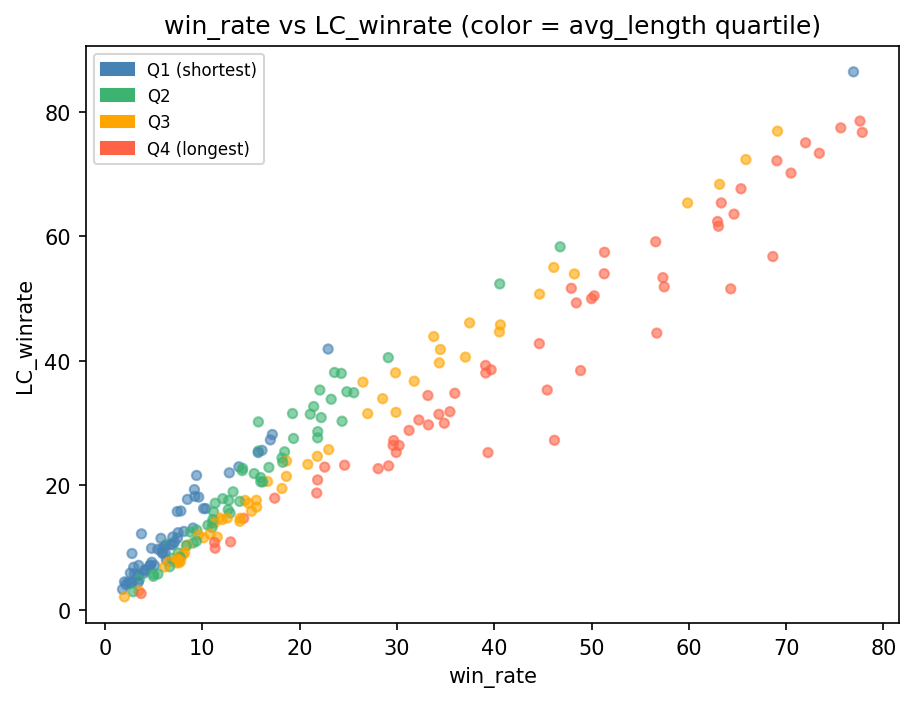
\includegraphics[width=\columnwidth]{figures/fig1_scatter_winrate_lc.png}
\caption{Scatter plot of win\_rate vs LC\_winrate with OLS regression line}
\label{fig:fig1_scatter_winrate_lc}
\end{figure}

\textit{Figure 1. Scatter plot of win\_rate vs LC\_winrate (N = 223 models, AlpacaEval 2.0) with OLS regression line. Spearman $\rho$ = 0.966 motivates the partial correlation analysis.}

\begin{figure}[htbp]
\centering
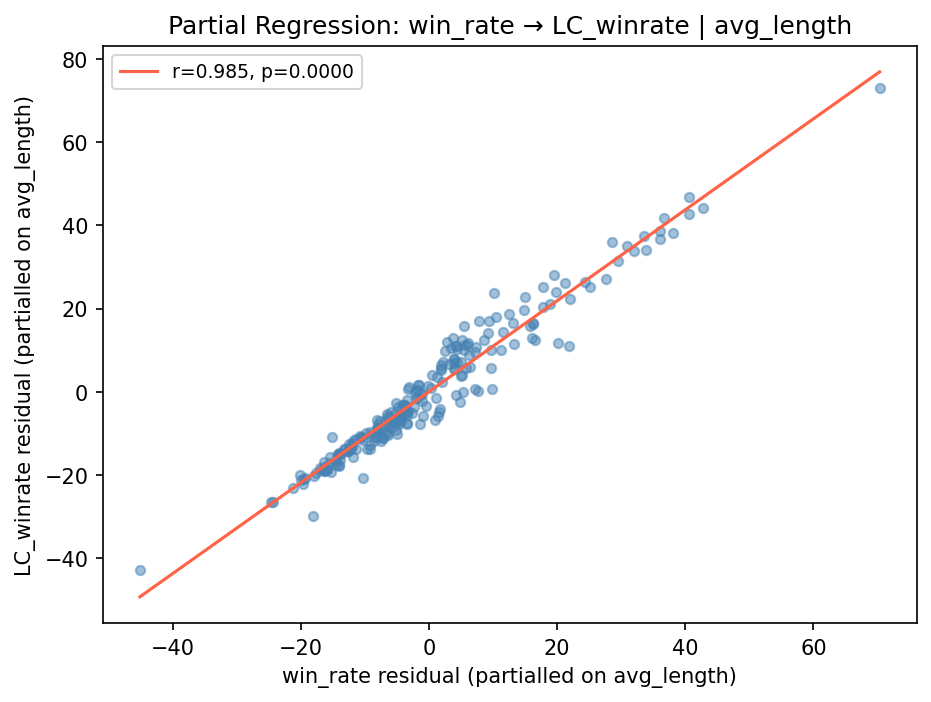
\includegraphics[width=\columnwidth]{figures/fig2_partial_regression.png}
\caption{Partial regression plot after controlling for avg\_length}
\label{fig:fig2_partial_regression}
\end{figure}

\textit{Figure 2. Partial regression plot: win\_rate vs LC\_winrate after controlling for avg\_length (residualized). Partial Spearman r = 0.9851 (p = 1.69e-170, one-tailed).}

\subsubsection{5.2 RQ2: Capability Dominates Verbosity in OLS (H-M1)}

In standardized OLS (LC\_winrate ~ win\_rate\_std + avg\_length\_std):

> \textbf{|$\beta _win|$ = 21.34 vs |$\beta _len|$ = 4.37 --- dominance ratio 4.88:1 (p\_win = 4.58e-145, p\_len = 8.02e-30)}

Full model $R^2$ = 0.963 (adjusted $R^2$ = 0.962) versus verbosity-only $R^2$ = 0.256 --- a difference of 70.7 percentage points attributable to the capability predictor.

$\beta _len = -4.37$ (negative): verbosity is penalized once capability is controlled, confirming the LC correction operates in the intended direction. Mild heteroscedasticity was detected (Breusch-Pagan p = 0.011); however, coefficient estimates remain unbiased and the significance of the capability coefficient (p\_win = 4.58e-145) is unaffected by this mild violation. Figure 6 shows the standardized coefficient comparison.

\begin{table}[htbp]
\centering
\resizebox{\columnwidth}{!}{%
\begin{tabular}{llll}
\toprule
Metric & Value &  &  \\
\midrule
\ & $\beta _win_std$\ &  & 21.34 \\
$\beta _len_std$ & $-4.37$ &  &  \\
Dominance ratio & 4.$88\times$ &  &  \\
Full model $R^2$ & 0.963 &  &  \\
Verbosity-only $R^2$ & 0.256 &  &  \\
$R^2$ gain from capability & +70.7 pp &  &  \\
Breusch-Pagan p & 0.011 (mild) &  &  \\
\bottomrule
\end{tabular}
}
\end{table}

\begin{figure}[htbp]
\centering
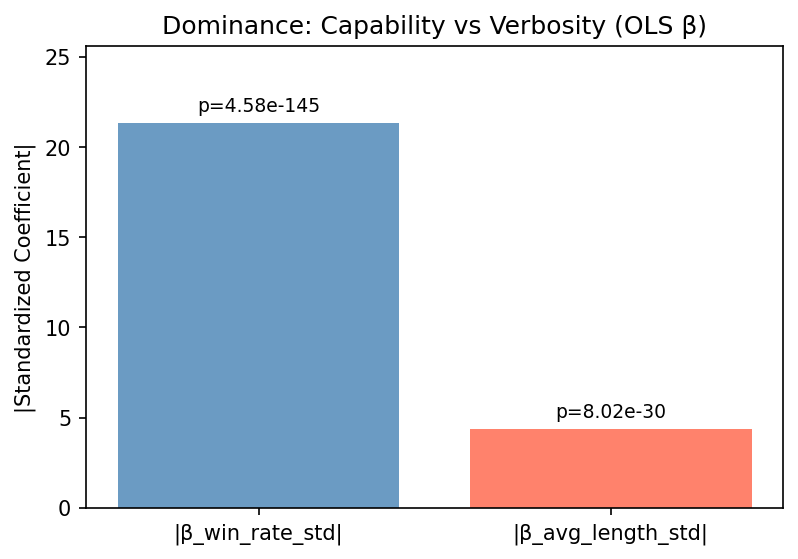
\includegraphics[width=\columnwidth]{figures/fig1_dominance_bar.png}
\caption{Standardized OLS coefficients bar chart}
\label{fig:fig1_dominance_bar}
\end{figure}

\textit{Figure 6. Standardized OLS coefficients: capability (|$\beta _win|$ = 21.34) vs verbosity (|$\beta _len|$ = 4.37). Dominance ratio 4.$88\times$; verbosity coefficient is negative after controlling capability.}

\subsubsection{5.3 RQ3: Estimator Robustness via FWL-Inspired Residualization (H-M2)}

> \textbf{$\rho_{resid}$ = 0.9739, p = 2.37e-144; delta = 0.0112 (< 0.02 ✓)}

Two independent estimators converge within 1.1 percentage points. Bootstrap 95\% CI on $\rho_{resid}$: [0.962, 0.981]. While the FWL theorem guarantees exact equality for Pearson OLS, the Spearman residualization here serves as an independent approximation; the 1.1 percentage point gap is well within expected sampling variation for N = 223, ruling out methodological artifact.

\begin{table}[htbp]
\centering
\resizebox{\columnwidth}{!}{%
\begin{tabular}{lll}
\toprule
Estimator & Value & p-value \\
\midrule
Pingouin partial\_corr (one-tailed) & 0.9851 & 1.69e-170 \\
FWL residual Spearman & 0.9739 & 2.37e-144 \\
Delta & 0.0112 & --- \\
Threshold met (delta < 0.02) & Yes & --- \\
\bottomrule
\end{tabular}
}
\end{table}

\begin{figure}[htbp]
\centering
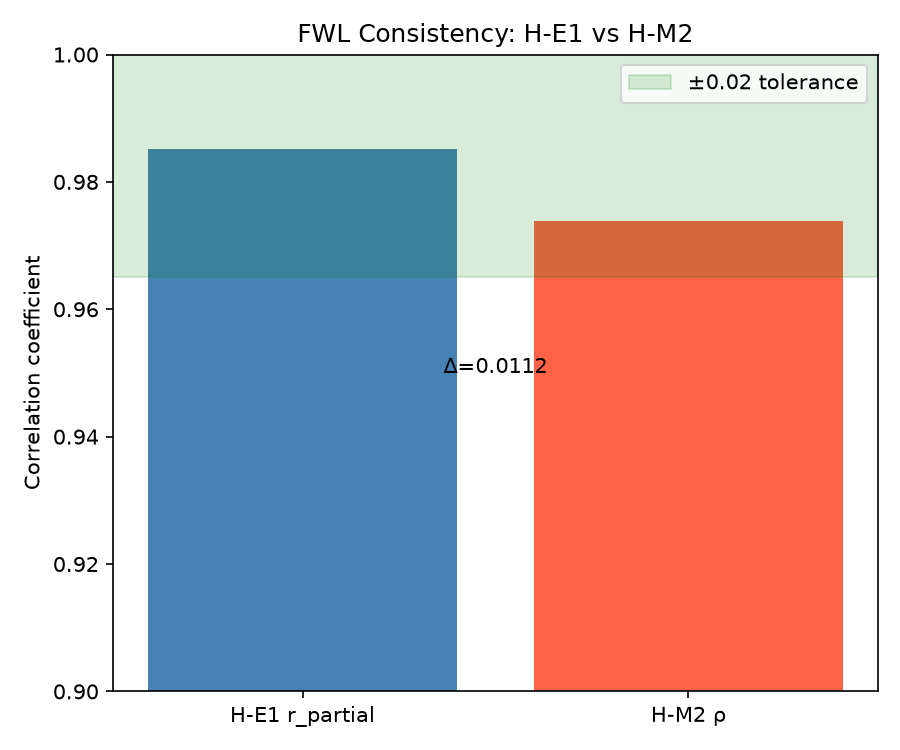
\includegraphics[width=\columnwidth]{figures/fig4_fwl_consistency.png}
\caption{FWL consistency comparison}
\label{fig:fig4_fwl_consistency}
\end{figure}

\textit{Figure 9. FWL consistency comparison: Pingouin partial corr (r = 0.9851) vs residual Spearman ($\rho$ = 0.9739). Delta = 0.011 < 0.02 threshold.}

\subsubsection{5.4 RQ4: LC Monotonicity Across Quartiles (H-C1)}

> \textbf{KW H = 196.32, p = 2.63e-42, $\epsilon ^2$ = 0.883 (large); Dunn Q1 vs Q4 p = 1.04e-38}
>
> \textbf{Monotonic: Q1 median = 7.14 < Q2 = 14.69 < Q3 = 26.41 < Q4 = 51.62}

$\epsilon ^2$ = 0.883 is a large effect by conventional thresholds (> 0.14 is considered large for Kruskal-Wallis $\epsilon ^{2})$. Q4 models show a 7.$2\times$ higher median LC\_winrate than Q1. Bootstrap 95% CI on Dunn Q1 vs Q4 p: [1.43e-40, 2.23e-35]. All pairwise adjacent quartile comparisons are statistically significant after Bonferroni correction (m = 6 pairs).

\begin{table}[htbp]
\centering
\resizebox{\columnwidth}{!}{%
\begin{tabular}{lll}
\toprule
Metric & Value & Status \\
\midrule
KW H & 196.32 & --- \\
KW p & 2.63e-42 & PASS \\
$\epsilon ^2$ & 0.883 & Large \\
Dunn Q1 vs Q4 Bonferroni p & 1.04e-38 & PASS \\
Monotonic ordering & True & CONFIRMED \\
Q4/Q1 median ratio & 7.$2\times$ & --- \\
\bottomrule
\end{tabular}
}
\end{table}

\begin{table}[htbp]
\centering
\resizebox{\columnwidth}{!}{%
\begin{tabular}{llll}
\toprule
Quartile & N & Median LC\_winrate & Mean LC\_winrate \\
\midrule
Q1 (win\_rate $\leq$ 5.19\%) & 56 & 7.14 & 7.44 \\
Q2 (5.19\%--14.29\%) & 56 & 14.69 & 14.85 \\
Q3 (14.29\%--27.85\%) & 55 & 26.41 & 27.75 \\
Q4 (win\_rate > 27.85\%) & 56 & 51.62 & 52.22 \\
\bottomrule
\end{tabular}
}
\end{table}

\begin{figure}[htbp]
\centering
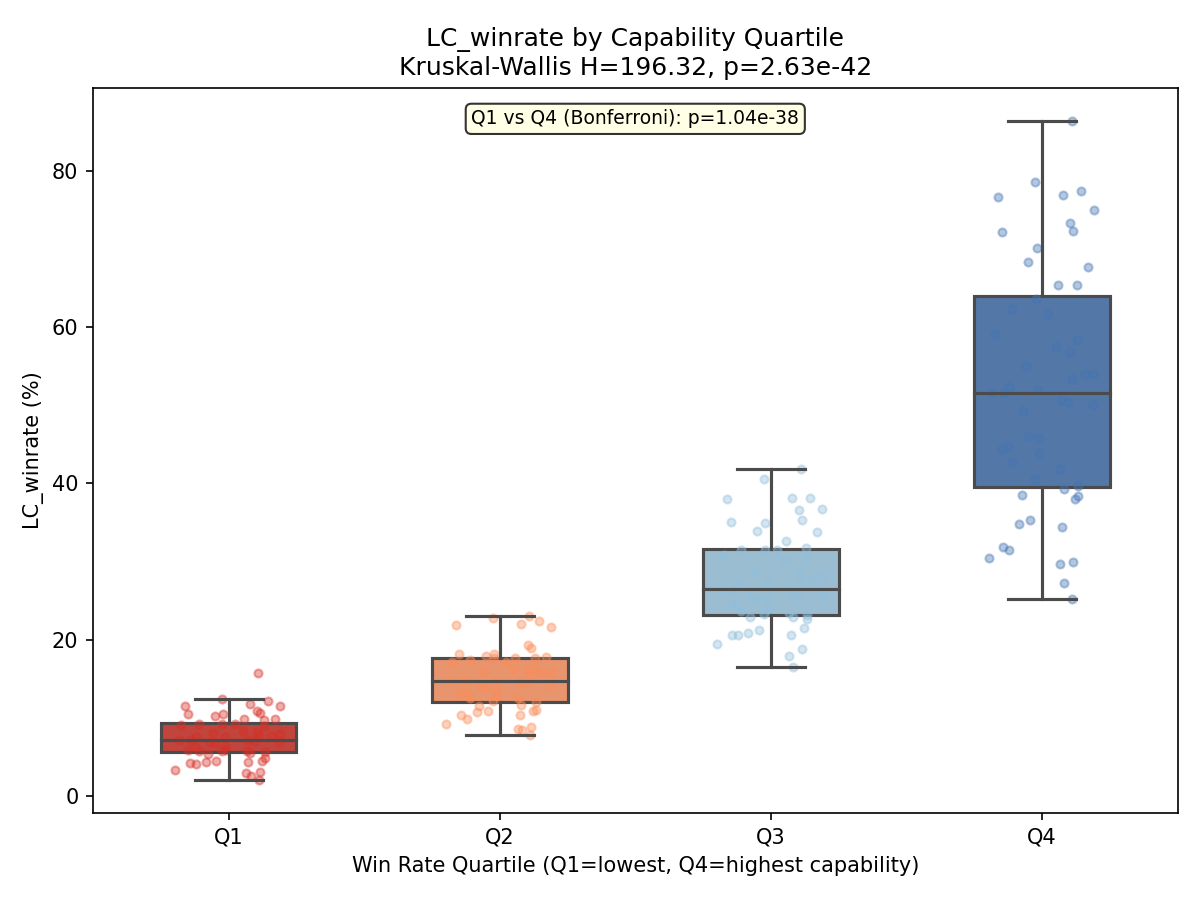
\includegraphics[width=\columnwidth]{figures/fig1_lc_winrate_boxplot.png}
\caption{Boxplot of LC\_winrate across capability quartiles}
\label{fig:fig1_lc_winrate_boxplot}
\end{figure}

\textit{Figure 11. Boxplot of LC\_winrate across capability quartiles (Q1--Q4). KW H = 196.32, p = 2.63e-42, $\epsilon ^2$ = 0.883 (large effect). Fully monotonic ordering.}

\subsubsection{5.5 RQ5: Alignment Gap $\Delta$ and Dependent Variable Choice (H-M3)}

Using $\Delta$ = LC\_winrate $-$ win\_rate as dependent variable:

> \textbf{KW H = 22.19, p = 5.97e-05, $\epsilon ^2$ = 0.088 (medium); Dunn Q1 vs Q4 Bonferroni p = 1.0 (non-significant)}
>
> \textbf{Non-monotonic: Q1 median $\Delta$ = 2.19, Q2 = 2.96, Q3 = 5.43, Q4 = 0.91}

The Kruskal-Wallis test on $\Delta$ is significant (p = 5.97e-05), confirming that the alignment gap varies across capability levels. However, the effect size is medium ($\epsilon ^2$ = 0.088), the quartile ordering is non-monotonic (Q4 < Q3), and the Dunn Q1 vs Q4 comparison is non-significant after Bonferroni correction (p = 1.0). The non-monotonic pattern in $\Delta$ is attributed to two factors: (1) mathematical dependency ($\Delta$ = LC\_winrate - win\_rate; grouping by win\_rate quartiles and testing $\Delta$ introduces self-referential structure); and (2) possible heterogeneity in verbosity strategies within Q3 models. Spearman $\rho$(win\_rate, $\Delta ) = -0.050$ (p = 0.455, non-significant), consistent with the mathematical dependency masking the bivariate relationship.

The effect-size contrast between H-M3 ($\epsilon ^2$ = 0.088) and H-C1 ($\epsilon ^2$ = 0.883) --- a $10\times$ difference --- illustrates the impact of dependent variable choice alone.

\begin{table*}[htbp]
\centering
\resizebox{\dimexpr 2\columnwidth+\columnsep\relax}{!}{%
\begin{tabular}{llllll}
\toprule
Dependent Variable & KW H & KW p & $\epsilon ^2$ & Monotonic & Dunn Q1 vs Q4 \\
\midrule
LC\_winrate & 196.32 & 2.63e-42 & 0.883 (large) & Yes & p = 1.04e-38 \\
$\Delta$ & 22.19 & 5.97e-05 & 0.088 (medium) & No & p = 1.0 (n.s.) \\
\bottomrule
\end{tabular}
}
\end{table*}

\begin{figure}[htbp]
\centering
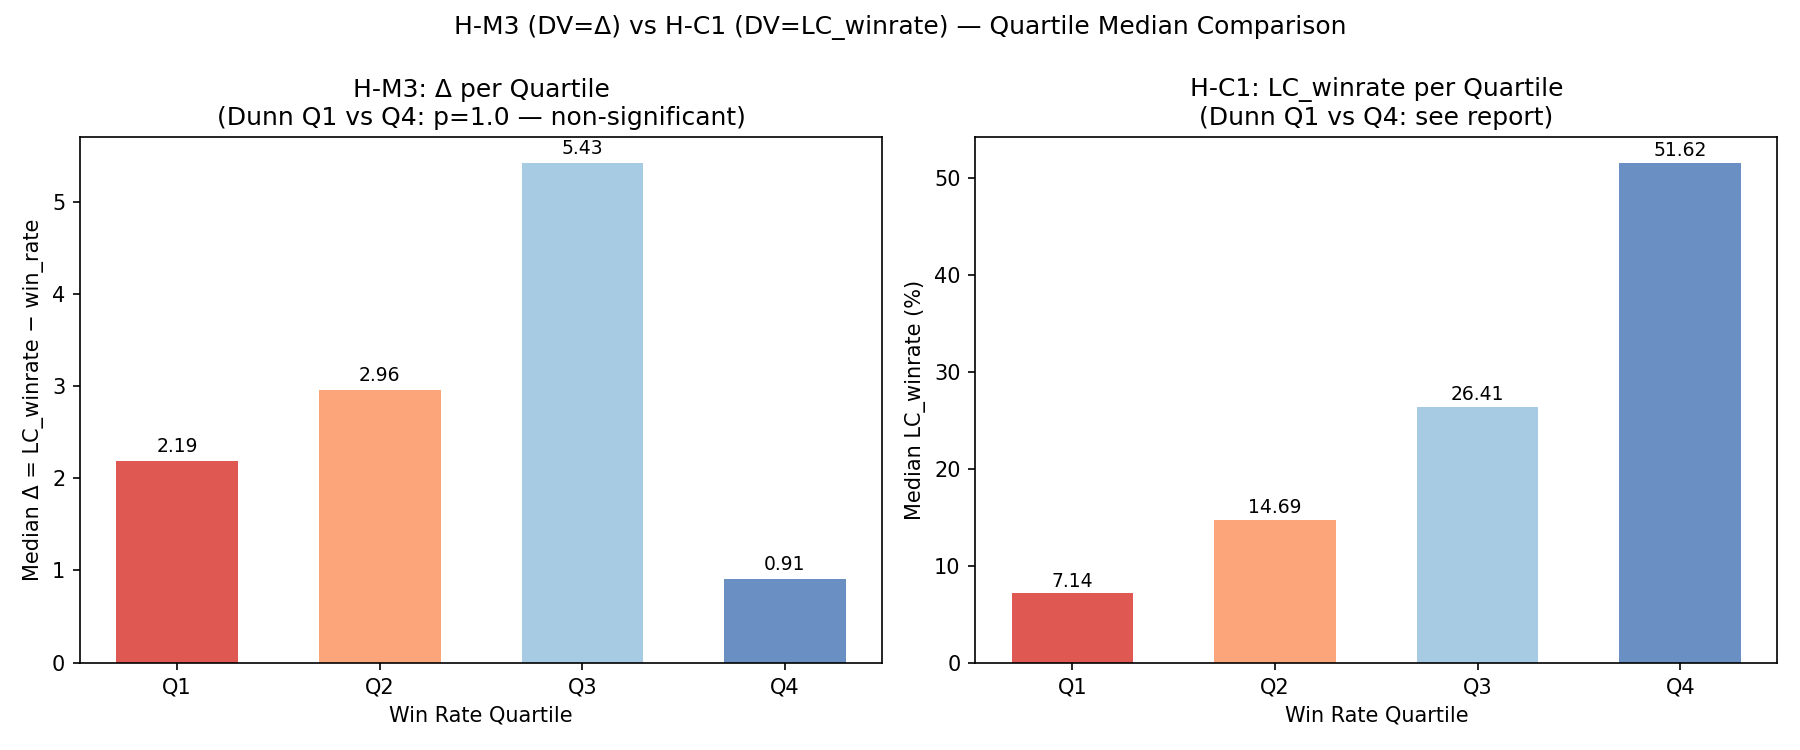
\includegraphics[width=\columnwidth]{figures/fig4_comparison_hm3_hc1.png}
\caption{Effect size comparison: $\epsilon ^2$ for H-M3 vs H-C1}
\label{fig:fig4_comparison_hm3_hc1}
\end{figure}

\textit{Figure 12. Effect size comparison: $\epsilon ^2$ = 0.088 (H-M3: KW on $\Delta )$ vs $\epsilon ^2$ = 0.883 (H-C1: KW on LC\_winrate). A $10\times$ difference from dependent variable choice alone.}

\subsubsection{5.6 Summary}

\begin{table*}[htbp]
\centering
\resizebox{\dimexpr 2\columnwidth+\columnsep\relax}{!}{%
\begin{tabular}{llllllll}
\toprule
Hypothesis & Gate & Result & Key Metric &  &  &  &  \\
\midrule
H-E1 & MUST\_WORK & PASS & r\_partial = 0.985; p = 1.69e-170 (one-tailed) &  &  &  &  \\
H-M1 & MUST\_WORK & PASS & \ & $\beta _win$\ & = 21.34 >> \ & $\beta _len$\ & = 4.37 \\
H-M2 & SHOULD\_WORK & PASS & delta = 0.011 < 0.02 &  &  &  &  \\
H-M3 & SHOULD\_WORK & PASS & KW p = 5.97e-05; Dunn Q1 vs Q4 p = 1.0 (n.s.) &  &  &  &  \\
H-C1 & SHOULD\_WORK & PASS & KW p = 2.63e-42; Dunn Q1 vs Q4 p = 1.04e-38 &  &  &  &  \\
\bottomrule
\end{tabular}
}
\end{table*}

